%% The first command in your LaTeX source must be the \documentclass command.
\documentclass[acmtog]{acmart}
\usepackage[english,ngerman]{babel}
\usepackage[utf8]{inputenc} 

%% \BibTeX command to typeset BibTeX logo in the docs
\AtBeginDocument{%
  \providecommand\BibTeX{{%
    \normalfont B\kern-0.5em{\scshape i\kern-0.25em b}\kern-0.8em\TeX}}}
    
\copyrightyear{2024}
\acmYear{2024}
\citestyle{acmauthoryear}

\usepackage[figurename=Fig.]{caption}
\setcopyright{none}
\makeatletter
\renewcommand{\fnum@figure}{Abb. \thefigure}
\makeatother
\addto\captionsngerman{\renewcommand{\figurename}{Abb.}}
\settopmatter{printacmref=false} % Removes citation information below abstract
\renewcommand\footnotetextcopyrightpermission[1]{} % removes footnote with conference information in first column

%%
%% end of the preamble, start of the body of the document source.
\begin{document}

%%
%% The "title" command has an optional parameter,
%% allowing the author to define a "short title" to be used in page headers.
\title{Sicherheitsaspekte in der (agilen) Softwareentwicklung}

%%
%% The "author" command and its associated commands are used to define
%% the authors and their affiliations.
%% Of note is the shared affiliation of the first two authors, and the
%% "authornote" and "authornotemark" commands
%% used to denote shared contribution to the research.
\author{Finn Hoedt}
\authornote{Alle Studierenden trugen zu gleichen Teilen zu dieser Arbeit bei.}
\author{Maurice Raymond Putzger}
\authornotemark[1]
\author{Bastian Wecke}
\authornotemark[1]
\affiliation{%
  \institution{Hochschule für Technik, Wirtschaft und Kultur Leipzig (HTWK Leipzig)}
  \streetaddress{Karl-Liebknecht-Str. 132}
  \city{Leipzig}
  %\state{Ohio}
  \country{Deutschland}
  \postcode{04277}
}
%%
%% By default, the full list of authors will be used in the page
%% headers. Often, this list is too long, and will overlap
%% other information printed in the page headers. This command allows
%% the author to define a more concise list
%% of authors' names for this purpose.
\renewcommand{\shortauthors}{Hoedt, Putzger und Wecke}

%%
%% The abstract is a short summary of the work to be presented in the
%% article.
\begin{abstract}
  (Abstract-Länge ist typischerweise 15-25 Zeilen lang, in der PDF-Darstellung) 
  
  
\end{abstract}

\maketitle

\section{Einleitung und Motivation}

(Beschreibung von Kontext, Problemen, Anforderungen und Zielen) 



(kurze Zusammenfassung der Struktur der Belegarbeit)

Diese Arbeit ist folgendermaßen strukturiert. 
In Kapitel ... 
...
...
Abschließend ...

\section{Grundlagen}

Im Folgenden werden Begriffe zu den Themen Sicherheit und Shift-Left in der Softwareentwicklung erklärt, um somit eine grundlegende Wissensbasis für die danach folgenden Kapitel zu schaffen.

Als \textit{sichere Software} definieren wir solche, die den grundlegenden Prinzipien der Informationssicherheit \cite{blakley_information_2001} entspricht und auch trotz verschiedener Widrigkeiten in ihrer Funktionalität zuverlässig bleibt \cite{oueslati_literature_2015}. Diese Prinzipien werden in folgende Kategorien unterteilt:
\begin{enumerate}
    \item \textbf{Vertraulichkeit} beschreibt den Schutz sensibler Daten vor unbefugtem Zugriff.
    \item \textbf{Integrität} stellt sicher, dass die Daten konsistent und unverändert bleiben, außer sie werden bewusst durch autorisierte Nutzer verändert.
    \item \textbf{Verfügbarkeit} garantiert, dass die Software und ihre genutzten Daten und Ressourcen stets zugänglich sind. Die Verfügbarkeit muss auch unter gezielten Angriffen gewährleistet werden.
    \item \textbf{Zuverlässigkeit} ist ein System dann, wenn es sich zu jedem Zeitpunkt erwartungsgemäß verhält. Dies gilt ebenfalls unter etwaigen Widrigkeiten, wie beispielsweise unbefugten Zugriffen von außen.
\end{enumerate}
Diese vier Prinzipien bilden die Grundlage für sichere Software und müssen somit bei der Entwicklung von sicherheitskritischen Prozessen gezielt beachtet werden.\

Der \textit{Shift-Left} Ansatz beschreibt das Verschieben von Prozeduren bzw. Aktivitäten aus späteren Phasen des Software Development Life Cycle in Frühere \cite{andriadi_impact_2023}. An einer zeitlichen Achse, wie sie in der Abbildung \ref{fig:shiftleft} zu sehen ist, kann man die Verschiebung nach Links erkennen. Die Abbildung zeigt, wie der Fokus von der Softwarequalität von einem späteren Zeitpunkt in einen Früheren verlagert wird. Dieses Vorgehen ist schon länger bekannt, doch der Name Shift-Left wurde durch \citet{smith_shift-left_2001} geprägt. Dieser sprach 2001 vom \textit{Shift-Left Testing} und erklärte, dass durch das frühere Testen in der Softwareentwicklung die Qualität der Software gesteigert und die Kosten von Fehlern gesenkt werden könne \cite{dawoud_better_2024}. Dafür müssten Quality Assurance (QA) und Entwickler parallel arbeiten, was zur Folge hätte, dass das QA-Team 1. nicht auf die Entwicklung warten muss und 2. entdeckte Fehler bereits während der Entwicklung direkt wieder beseitigt werden können \cite{andriadi_impact_2023}. 

\begin{figure}
    \centering
    
\includegraphics[width=0.9\linewidth]{images/Shift_Left.png}
    \caption{Shift-Left Verschiebung von Fokus auf Qualität im Software Development Life Cycle}
    \label{fig:shiftleft}
  \end{figure}

Mit \textit{Shift-Left Security} ist die Anwendung des Shift-Left Gedanken auf den Bereich der Software-Security gemeint \cite{dawoud_better_2024}. Viele Sicherheitsprozesse werden in der Regel erst am Ende der Entwicklung durchgeführt, wodurch Fehler oder Sicherheitslücken oft zu spät erkannt werden \cite{dawoud_better_2024}. Durch Shift-Left Security werden jene Prozesse in die früheren Phasen des Software Development Cycles verschoben, wodurch Bedrohungen zeitnah erkannt und beseitigt werden können.

\textit{Development, Security and Operations (DevSecOps)} beschreibt die Erweiterung des klassischen \textit{DevOps} durch die Einbindung von Security Aspekten \cite{rajapakse_challenges_2022}. Die Aufgabe des DevSecOps ist es, Sicherheitspraktiken in den gesamten Entwicklungszyklus einzubinden, um so die Sicherheit der Software zu gewährleisten. Dabei werden automatisierte Sicherheitstest kontinuierlich angepasst und ausgewertet, wodurch die Sicherheit gewährleistet wird, sowie auch Zeit und Kosten gespart werden. DevSecOps zielt ebenfalls darauf ab, die Zusammenarbeit und Kommunikation von Entwicklern, Sicherheitsexperten und Betriebsteams zu verbessern, um ein Verständnis von Sicherheit im ganzen Team zu bilden \cite{rajapakse_challenges_2022}.




\section{(Hauptteil mit ggf. mehreren Sections)}

(der Hauptteil umfasst typischerweise ca. 2/3 bis 3/4 des Texts der Arbeit.)

\subsection{Shift-Left Modelle}
Der Shift-Left-Gedanke ist eine grundsätzliche Herangehensweise, die sich auf die meisten Konzepte und Modelle anwenden lässt. Da dieser Beitrag sich auf die Verbindung von agilen Methoden und Security durch den Shift-Left-Ansatz konzentriert, werden im Folgenden zwei Shift-Left-Modelle erklärt, die dabei behilflich sind.

\begin{figure}
    \centering
    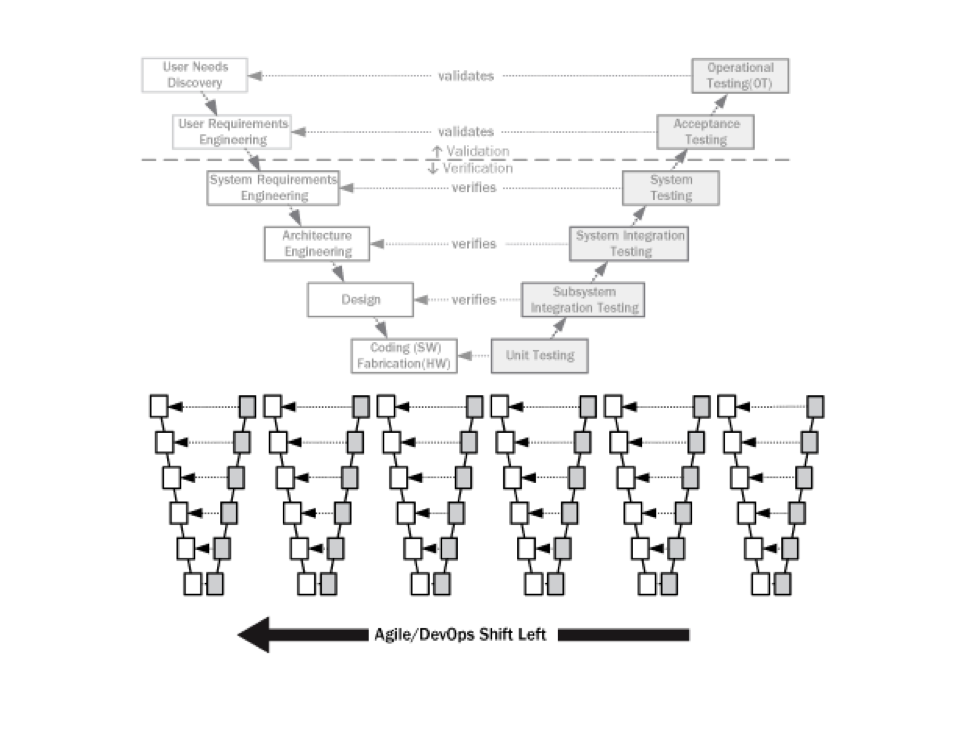
\includegraphics[width=0.9\linewidth]{images/Agile_DevOps_Shift_Left.png}
    \caption{Agile/DevOps Shift Left (Quelle: )}
    \label{fig:agiledevops}
\end{figure}

Das erste Modell ist das \textit{Agile/DevOps Shift-Left-Testing}. Zur Erklärung des Modells dient die Abbildung \ref{fig:agiledevops}. Ausgangslage für die Grafik ist das traditionelle V-Modell, welches verblasst in der oberen Hälfte von Abbildung \ref{fig:agiledevops} zu erkennen ist. Die mehrfachen Vs darunter visualisieren die Arbeitsweise im agilen Bereich. Jedes V stellt einen Zyklus der Entwicklung dar, der beim agilen Arbeiten meist \textit{Sprint} genannt wird \cite{rani_shift-left_2023}. Diese Aufteilung nutzt bereits eine Implementierung des Shift-Left-Ansatzes. Durch das Aufteilen eines gesamten Projekts in mehrere kleine Zyklen werden beispielsweise Tests in jedem Zyklus umgesetzt \cite{rani_shift-left_2023}. Betrachtet man die gesamte Laufzeit eines Projekts, werden Tests dadurch automatisch nicht erst am Ende des gesamten Projekts umgesetzt \cite{bjerke-gulstuen_high_2015}. Agile/DevOps Shift-Left-Testing schlägt weiterhin vor, den Fokus auf das Testing in frühere Sprints zu verstärken \cite{bjerke-gulstuen_high_2015}. Dabei ist das Automatisieren dieser Tests ein ausschlaggebendes Prinzip im DevOps-Bereich \cite{rani_shift-left_2023}. Shift-Left will diese Automatisierung nutzen, um das kontinuierliche Testen bereits als Bestandteil in die frühen Entwicklungsphasen zu integrieren \cite{rani_shift-left_2023}. Die frühzeitige Nutzung von CI/CD und DevOps hilft dabei, Bugs und Sicherheitslücken rechtzeitig zu erkennen und somit langfristige Kosten zu sparen \cite{rani_shift-left_2023}. Eine effektive Methode, um Tests für Sicherheitslücken bzw. -probleme zu automatisieren, ist die Nutzung von SAST und DAST, welche später noch genauer analysiert werden. Eine weitere Eigenschaft, die durch die agile Herangehensweise und Shift-Left gestärkt wird, ist die Zusammenarbeit und Kommunikation zwischen Development- und Testing-Teams \cite{rani_shift-left_2023}. Durch die Parallelisierung beider Prozesse gibt es einen höheren Austausch von Feedback, wodurch auf Fehler schnell reagiert werden kann. Vor allem bei Projekten mit hohen Sicherheitsanforderungen wird dadurch das Bewusstsein für Sicherheit bei allen Beteiligten gestärkt \cite{dawoud_better_2024}.

Der zweite Ansatz, der hier vorgestellt werden soll, ist das \textit{Model-Based Shift-Left Testing (MBSLT)}. Wie zuvor veranschaulicht Abbildung \ref{fig:modelbased} die Herangehensweise für das MBSLT basierend auf dem V-Modell. Anders als der Agile/DevOps-Ansatz fokussiert sich MBSLT auf das Testen des gesamten Modells und nicht auf den Quellcode an sich \cite{rani_shift-left_2023}. In \ref{fig:modelbased} ist zu erkennen, dass neben jedem standardmäßigen Schritt des V-Modells ein paralleler Schritt erfolgt, der darauf abzielt, das Systemmodell zu testen. Diese Systemmodelle werden beispielsweise durch UML oder Datenflussdiagramme dargestellt \cite{rani_shift-left_2023}. Basierend darauf werden Tests erstellt, um Schwachstellen in der Architektur- und Design-Ebene zu erkennen. Auch diese Art von Tests kann durch CI/CD automatisiert werden \cite{rani_shift-left_2023}. MBSLT hilft dabei, potenzielle Fehler noch vor der Implementierung zu erkennen, wodurch später Kosten vermieden werden können \cite{rani_shift-left_2023}. Des Weiteren wird die Anforderungsanalyse verbessert, da MBSLT sicherstellt, dass Anforderungen vollständig und konsistent sind \cite{rani_shift-left_2023}. Dieser Vorteil trägt somit auch zur besseren Kommunikation zwischen dem Development- und dem Testing-Team bei.


\begin{figure}
    \centering
    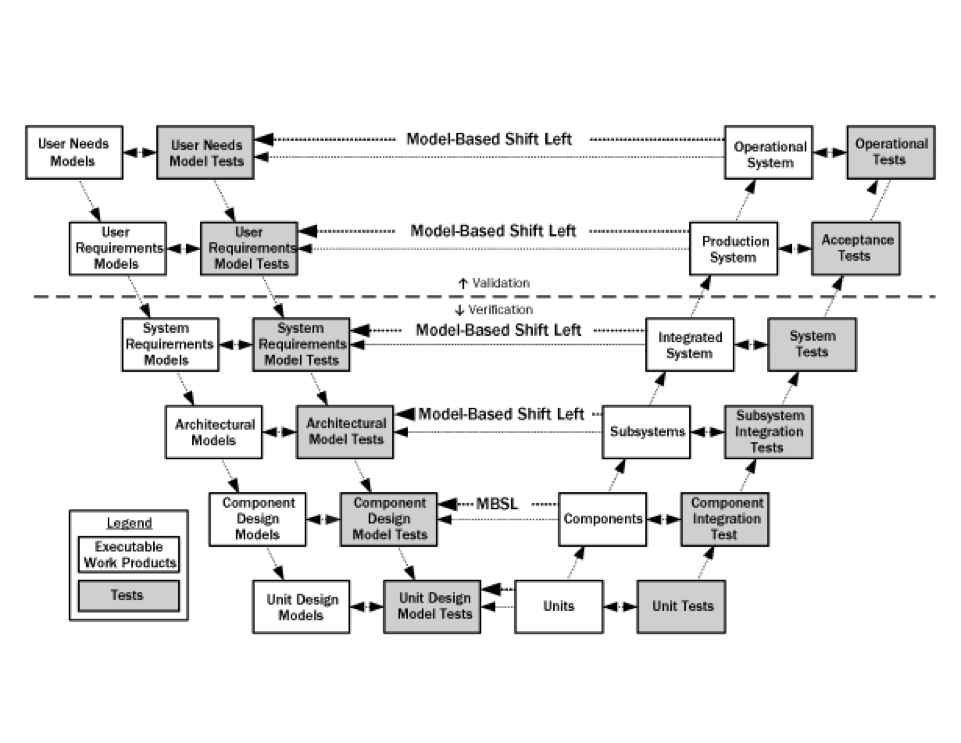
\includegraphics[width=0.9\linewidth]{images/Model_Based_Shift_Left.png}
    \caption{Model-Based Shift Left (Quelle: )}
    \label{fig:modelbased}
\end{figure}

\subsection{Herausforderungen}
In der modernen Softwareentwicklung finden agile Methoden wie Scrum zunehmende Anwendung.
Diese Vorgehensweisen versprechen in der Regel eine gesteigerte Produktivität, bessere Produktqualität sowie eine erhöhte Kundenzufriedenheit. 
Sie zeichnen sich insbesondere durch häufige Änderungen der Anforderungen und kontinuierliche Releases aus.
Sicherheitsaspekte sind allerdings in den gängigen agilen Praktiken nicht systematisch verankert. Das erschwert die Entwicklung sicherer Software. \cite{oueslati_literature_2015}

Im Folgenden werden die wesentlichen Herausforderungen bei der Integration von Sicherheitsanforderungen in agile Entwicklungsprozesse erläutert. 

Die Probleme erstrecken sich über verschiedene Phasen des Software Development Life Cycle (SDLC).
Ein zentrales Prinzip agiler Methoden ist die kontinuierliche Lieferung von Software. 
Das bedeutet, dass in jeder Iteration sämtliche SDLC-Aktivitäten durchlaufen werden müssen.
Das beinhaltet alle sicherheitsrelevanten Praktiken. 
Da Iterationen jedoch oft nur wenige Wochen umfassen, ist es schwierig, zeitintensive Sicherheitsmaßnahmen in diesen kurzen Zyklen durchzuführen. \cite{oueslati_literature_2015}

Darüber hinaus resultieren weitere Herausforderungen aus dem inkrementellen Vorgehen sowie dem Streben nach technischer Exzellenz. 
Das wird in agilen Methoden unter anderem durch häufiges Refactoring verwirklicht. 
Die Refactorings können jedoch bestehende Sicherheitsanforderungen versehentlich verletzen. 
Zusätzlich führt die hohe Priorität, kurzfristige Kundenwünsche umzusetzen, zu Designänderungen.
Diese können bestehende Sicherheitsvorgaben brechen und erschweren Sicherheitsmaßnahmen wie Code Reviews. \cite{oueslati_literature_2015}

Ein weiterer Problembereich betrifft die Qualität der Dokumentation.
Nach den agilen Werten hat funktionierende Software Vorrang gegenüber umfassender Dokumentation. 
Diese Herangehensweise kann zu lückenhafter oder unvollständiger Dokumentation führen.
Sicherheitskonzepte erfordern aber in der Regel eine detaillierte und verlässliche Dokumentationsbasis.
Tests decken zudem häufig nur die Funktionalität ab und überprüfen somit primär positive Anforderungen.
Sicherheit hingegen umfasst zumeist negative Anforderungen, bei denen es darum geht, Fehlverhalten oder Schwachstellen zu erkennen.
Da klassische Akzeptanztests hierfür nur bedingt geeignet sind, bleiben potenzielle Sicherheitslücken oft verborgen. \cite{oueslati_literature_2015}

Des Weiteren entsteht ein Konflikt im Hinblick auf Audits. 
Agile Methoden sehen einen kontinuierlichen Verbesserungsprozess des Entwicklungsprozesses vor. 
Audits hingegen verlangen meist einen stabilen, über längere Zeiträume unveränderten Prozess. 
Dadurch wird Nachvollziehbarkeit und Vergleichbarkeit gewährleistet.
Dies erschwert die Einhaltung auditrelevanter Standards in hochflexiblen agilen Umgebungen. \cite{oueslati_literature_2015}

Das Sicherheitsbewusstsein und die Zusammenarbeit innerhalb des Teams stellen eine weitere Herausforderung dar.
Der Projektfortschritt wird in agilen Prozessen vorwiegend an funktionsfähiger Software gemessen.
Dadurch rücken Sicherheitsaspekte in den Hintergrund. 
Darüber hinaus wird empfohlen, sicherheitstechnische Bewertungen unabhängig von den Entwicklerteams durchzuführen. 
Somit wird der Einfluss sozialer Beziehungen auf die Ergebnisse vermieden.
Dies steht jedoch im Widerspruch zu den agilen Prinzipien, die auf enger Kooperation und fortlaufendem Austausch basieren. \cite{oueslati_literature_2015}

Schließlich hat auch das Sicherheitsmanagement mit den kurzen Iterationen und dem Fokus auf die Bereitstellung neuer Funktionalitäten zu kämpfen. 
Umfangreiche Sicherheitsaktivitäten erhöhen die Entwicklungskosten und erfordern zusätzliche Ressourcen.
Dazu kommt, dass die Sicherheitsmaßnahmen häufig nicht für die laufende Anwendung erforderlich sind.
In vielen Fällen wird daher zugunsten schnellerer Releases auf umfassende Sicherheitsmaßnahmen verzichtet. \cite{oueslati_literature_2015}
 

\subsection{Static Application Security Testing (SAST)}
SAST-Werkzeuge führen eine ''White-Box''-Analyse durch, bei der der Quellcode direkt auf potenzielle Sicherheitslücken untersucht wird.
Die Anwendung muss hierfür nicht ausgeführt werden. 
Durch die frühzeitige Erkennung von Sicherheitslücken in der Entwicklungsphase tragen SAST-Tools maßgeblich dazu bei, potenzielle Schwachstellen proaktiv zu beheben. 
Typische Beispiele für SAST-Werkzeuge sind Fortify SCA und FindSecurityBugs. \cite{mateo_tudela_combining_2020}


\subsection{Dynamic Application Security Testing (DAST)}
DAST-Werkzeuge folgen einem ''Black-Box''-Ansatz, da sie Angriffe von außen auf die laufende Anwendung simulieren.
Auf diese Weise lassen sich Sicherheitslücken identifizieren, die erst während der Laufzeit auftreten. DAST-Tools untersuchen primär Schnittstellen einer ausgeführten Anwendung und erfordern keine Kenntnisse über den zugrunde liegenden Quellcode. 
Daher sind sie in der Regel unabhängig von der verwendeten Programmiersprache. 
Bekannte Beispiele für DAST-Werkzeuge sind OWASP ZAP und Arachni. \cite{mateo_tudela_combining_2020}

\subsection{Interactive Application Security Testing (IAST}
IAST wird, ähnlich wie SAST, dem ''White-Box''-Ansatz zugeordnet, kombiniert jedoch Elemente aus SAST und DAST zu einem hybriden Verfahren. 
Dabei überwachen und analysieren die IAST-Werkzeuge den Quellcode während der Ausführung, was eine präzise Sicherheitsprüfung anhand realer Laufzeitinformationen ermöglicht. 
IAST-Werkzeuge sind direkt auf dem Server integriert sind, weshalb sie mit der jeweiligen Programmiersprache kompatibel sein müssen. 
Da sie ausschließlich serverseitige Analysen durchführen, sind sie nicht in der Lage, clientseitige Sicherheitslücken aufzudecken. Bekannte Beispiele für IAST-Werkzeuge sind Contrast und CxIAST. \cite{mateo_tudela_combining_2020}



\subsection{Effektivität von Application Security Testing}

\begin{figure}[H]
	\centering
	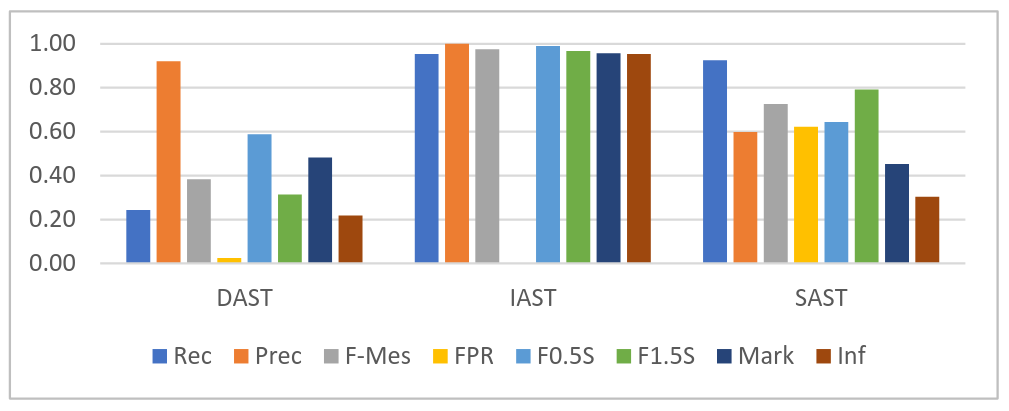
\includegraphics[width=0.9\linewidth]{images/AST_Comparison.png}
	\caption{AST Vergleich ohne Kombination}
	\label{fig:astCompare}
\end{figure}


\begin{figure}[H]
	\centering
	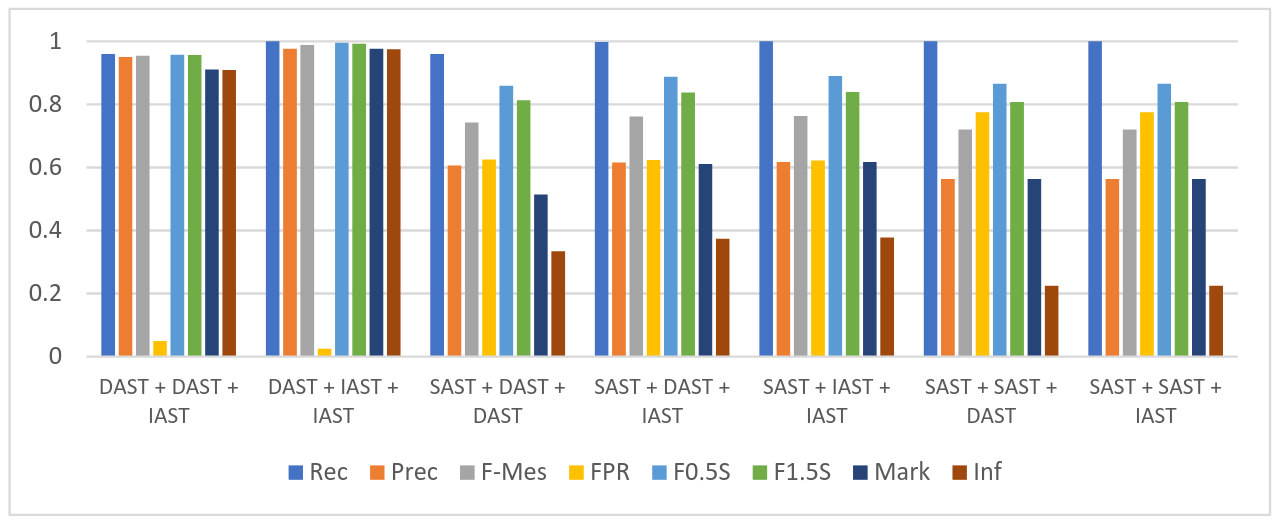
\includegraphics[width=0.9\linewidth]{images/AST_Comparison_Combination.png}
	\caption{AST Vergleich mit Kombination}
	\label{fig:astCompareCompination}
\end{figure}

\subsection{Scrum for Safety}

\textit{Scrum for Safety} zielt darauf ab, die Innovationsfähigkeit und Effizienz agiler Methoden mit den strengen Anforderungen an Sicherheit und Konformität zu vereinen. 
Zu diesem Zweck führt es spezifische Rollen, Prinzipien und Workflows ein, um die Qualität und Sicherheit der zu entwickelnden Software zu gewährleisten. 
Das Framework erweitert die klassischen Scrum-Rollen um zusätzliche Rollen, die in sicherheitskritischen Projekten erforderlich sind. \cite{barbareschi_scrum_2022} Dazu zählen: 

\begin{enumerate}
  \item \textbf{Verifikator:} Verantwortlich für die Überprüfung der Verifikationstests.
  \item \textbf{Validator:} Bestätigt, dass die Anforderungen korrekt und vollständig umgesetzt wurden.
  \item \textbf{Assessor:} Externe Person, die sicherstellt, dass der Entwicklungsprozess den geltenden Standards entspricht.
\end{enumerate}

Die zusätzlichen Rollen sind dafür zuständig, 
die Unabhängigkeit der Prüfprozesse zu gewährleisten und die Erfüllung der Anforderungen an die Softwarequalität sicherzustellen. \cite{barbareschi_scrum_2022}

Neben der Integration zusätzlicher Rollen werden im Rahmen von \textit{Scrum for Safety} auch neue Konzepte eingeführt, die darauf abzielen, die Sicherheit der Softwareentwicklung zu gewährleisten. 
Hierzu zählt das Sprint-Hardening, dessen Zielsetzung darin besteht, die Bereitstellung einer validierten Softwareversion am Ende jeder Iteration sicherzustellen. In jeder Iteration wird demnach darauf geachtet, 
dass Benutzerdokumentationen und Konformitätsnachweise erstellt werden, die dann für die externe Softwarebewertung verwendet werden können. \cite{barbareschi_scrum_2022}
Ein weiteres Konzept ist die Continuous Compliance. Das beinhaltet die kontinuierliche Durchführung von Verifizierungs- und Validierungsaktivitäten, sodass die Software jederzeit konform ist. 
Das Ziel dieses Ansatzes ist die frühzeitige Erkennung und Behebung kritischer Fehler. \cite{barbareschi_scrum_2022} Das dritte Konzept ist die Living Traceability.
Die Einführung einer klaren Rückverfolgbarkeit in jedem Prozess bei der Umsetzung von Benutzeranforderungen zielt darauf ab, die Zertifizierung der Software durch externe Prüftstellen zu erleichtern. \cite{barbareschi_scrum_2022}

Der zentrale Prozess in \textit{Scrum for Safety} wird als Safe-Sprint bezeichnet. In Anlehnung an das klassische Scrum-Prinzip stellt der Safe-Sprint eine zeitlich begrenzte Iteration dar, in der ein neues Software-Inkrement entwickelt wird. 
Im Gegensatz zum klassischen Scrum wird dabei sichergestellt, dass das entwickelte Inkrement durch die eingeführten Konzepte sicherheitstechnisch validiert ist. \cite{barbareschi_scrum_2022}
\textit{Scrum4Safety} setzt zu diesem Zweck bereits in der Planungsphase mit dem Safe-Sprint an und integriert Safety-Stories neben den klassischen User-Stories in den Backlog.
Das Ziel dieser Vorgehensweise ist die Gewährleistung der Berücksichtigung von Sicherheit bereits in der Anforderungsphase. 
Eine weitere Maßnahme zur Sicherstellung der Berücksichtigung von Sicherheit in der Anforderungsphase ist die frühzeitige Einbindung von Sicherheitsüberprüfungen und Testphasen im Ablauf des Safe-Sprints. \cite{barbareschi_scrum_2022}

In sicherheitskritischen Projekten nimmt die Dokumentation eine zentrale Rolle ein. Aus diesem Grund wird in den Ablauf eines Safe-Sprints eine Dokumentationsphase integriert (siehe Abbildung \ref{fig:scrum4safety}). 
Dabei wird Dokumentation nicht als Haupttreiber des Prozesses betrachtet, sondern als Resultat jeder Iteration. \cite{barbareschi_scrum_2022}
Das Ziel besteht darin, unnötigen Dokumentationsaufwand zu vermeiden und ausschließlich die für die Zertifizierung erforderlichen Dokumente zu erstellen. 
\textit{Scrum for Safety} schlägt zur Erstellung von Dokumentationen zusätzlich noch automatisierte Tools vor, wie Doxygen oder IBM DOORS, um Dokumente automatisch aus dem Code zu generieren und den Aufwand zusätzlich zu minimieren. \cite{barbareschi_scrum_2022}

Im Rahmen der Evaluierung von \textit{Scrum for Safety} wurde eine Fallstudie mit Rete Ferroviaria Italiana (RFI) durchgeführt. Gegenstand der Fallstudie war die Entwicklung einer sicheren Middleware für die Kommunikation zwischen Eisenbahnsignalsystemen. 
Die Herausforderung bestand darin, bestehende Hardware und Protokolle zu unterstützen, um eine nahtlose Integration in vorhandene Systeme zu gewährleisten. Ein weiterer Aspekt, den es zu berücksichtigen galt, 
war die Sicherstellung der Zuverlässigkeit und Sicherheit der Systeme, um potenzielle Gefahrenquellen zu minimieren und die Einhaltung gesetzlicher Vorgaben sowie branchenspezifischer Richtlinien zu gewährleisten. Die Fallstudie ergab, 
dass die Integration umfangreicher Sicherheitsmaßnahmen in kurze Iterationen eine Herausforderung darstellte. \cite{barbareschi_scrum_2022}
Aus diesem Grund wurde die Länge der Iterationen auf vier Wochen erweitert, wobei etwa 75 \% der Sprintzeit für Verifikation und Validierung verwendet wurde.Dies zeigte sich insbesondere bei der Fehlererkennung, 
da die implementierten Sicherheitsmaßnahmen maßgeblich dazu beitrugen, Fehler frühzeitig zu erkennen und zu beheben. 
Die Implementierung von Dokumentationsmaßnahmen trug ebenfalls zur Nachvollziehbarkeit der Entwicklungsaktivitäten bei und erleichterte dadurch die Zertifizierung durch externe Prüfstellen. \cite{barbareschi_scrum_2022}

\begin{figure}
  \centering
  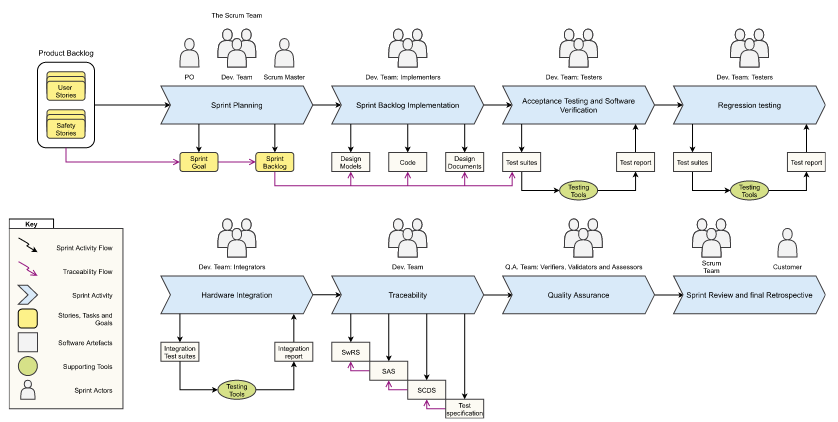
\includegraphics[width=0.9\linewidth]{images/S4S-Safe-Sprint.png}
  \caption{Scrum for Safety Prozess}
  \label{fig:scrum4safety}
\end{figure}

\subsection{Security Standard Compliant Scaled Agile Framework}

\textit{$S^2$C-SAFe} ist ein Framework, das auf dem \textit{Scaled Agile Framework (SAFe)} basiert und speziell für sicherheitskritische Projekte entwickelt wurde. 
Dafür erweitert es das klassische SAFe um Sicherheitsanforderungen aus dem Standard IEC 62443-4-1, der Richtlinien für die sichere Produktentwicklung
in industriellen Umgebungen. \cite{moyon_how_2020} Das Ziel ist es, agile Entwicklungsprozesse mit Sicherheitsstandards zu verbinden und dadurch eine kontinuierliche Sicherheitsüberprüfung zu gewährleisten (siehe Abbildung \ref{fig:s2c}), ohne 
die Flexibilität und Geschwindigkeit der Entwicklung zu beeinträchtigen. \cite{moyon_how_2020}

\textit{$S^2$C-SAFe} implementiert das Konzept \textbf{Continuous Security}, dessen Ziel die Integration von Sicherheit als fundamentalem Aspekt in sämtliche Prozesse ist. 
Ziel ist es, Sicherheit von einer nicht-funktionalen Anforderung zu einer integralen Komponente der Softwareentwicklung zu machen.
Dieses wird bereits in der Planungsphase implementiert, in welcher Sicherheitsanforderungen systematisch in den Backlog integriert werden (siehe Abbildung \ref{fig:s2c}). \cite{moyon_how_2020} 
Hierbei werden Product Owner und Systemarchitekten gezielt in Sicherheitsaspekte eingebunden und entsprechend geschult, um von Anfang an ein hohes Sicherheitsbewusstsein zu gewährleisten. 
In der Implementierungsphase werden die Sicherheitsanforderungen durch teamübergreifende Coding-Standards umgesetzt und als fester Bestandteil in die Definition of Done integriert. 
Dies gewährleistet, dass Sicherheitsaspekte bei jeder Entwicklung berücksichtigt werden. \cite{moyon_how_2020}
Die Qualitätssicherung erfolgt durch dedizierte Verifikations- und Validierungsmaßnahmen, die von unabhängigen Security Experts durchgeführt werden. 
Ein wesentliches Merkmal des Continuous Security Ansatzes ist dabei die kontinuierliche Durchführung expliziter Sicherheitsanforderungen und Tests, wodurch Sicherheitsmaßnahmen nicht als einmaliger Check, 
sondern als fortlaufender Prozess verstanden werden. \cite{moyon_how_2020}

\textit{$S^2$C-SAFe} wurde in einer Fallstudie bei Siemens getestet, welche dann durch Interviews mit 16 Experten aus dem Siemens-Umfeld evaluiert wurde.
Die Experten stammen aus verschiedenen Bereichen, darunter Sicherheitsstandards, agile Entwicklung und Compliance. Aus den Interview ergab sich, dass das Framework als praktikabel angesehen wird,
um die Diskrepanz zwischen agilen Methoden und Sicherheitsanforderungen zu überbrücken. Zudem erwies sich die Visualisierung der Prozesse, welche bei der Entwicklung von \textit{$S^2$C-SAFe} erstellt wurden, als hilfreich, 
um eine gemeinsame Sprache zwischen Sicherheits- und Entwicklungsteams zu schaffen. Neben den Vorteilen, die das Framework für die Integration von Sicherheitsanforderungen in agile Prozesse bietet, blieben jedoch auch Herausforderungen bestehen.
Gerade die fehlende Sicherheitsexpertise in agilen Teams führte zu Schwierigkeiten bei der Umsetzung von Sicherheitsanforderungen. Dies zeigte siche bei der Priorisierung von Sicherheitsanforderungen, wobei oft unklar war, 
welche Sicherheitsmaßnahmen am dringendsten umgesetzt werden sollten. Auch die unterschiedliche Interpretation von Sicherheitsanforderungen durch Entwickler und Sicherheitsexperten stellte eine Herausforderung dar, was zu Missverständnissen und Fehlern führen könnte. Als Lösung schlagen die Autoren vor,
spezielle Rollen wie einen Security Product Owner oder einen Secure System Architect einzuführen, um die Kommunikation zwischen den Teams zu verbessern und die Umsetzung von Sicherheitsanforderungen zu erleichtern. 
Eine weitere Herausforderung war die Komplexität der Sicherheitsanforderungen, da die Integration der Maßnahmen in die kurzen Entwicklungszyklen herausfordernd war. 



\begin{figure}
  \centering
  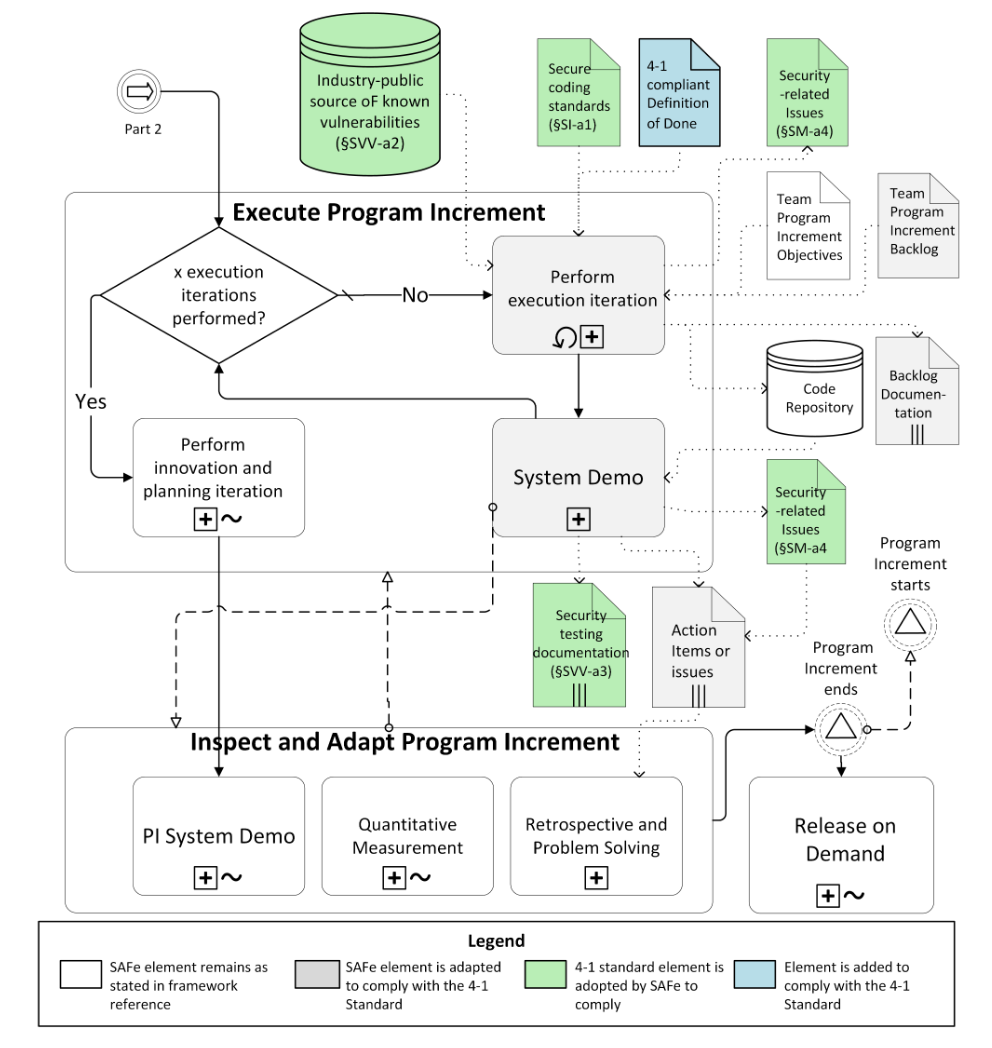
\includegraphics[width=0.9\linewidth]{images/S2C.png}
  \caption{Security Standard Compliant Scaled Agile Framework}
  \label{fig:s2c}
\end{figure}











\section{Diskussion}

(Einordnung, Interpretation und Bewertung der Erkenntnisse -- (nachvollziehbare, begründbare) Meinungen sind erlaubt) 



\section{Zusammenfassung und Ausblick}

(Überblick über die gesamte Arbeit, Rückführung auf Aussagen aus Kapitel 1 durchführen, offene Punkte als neue Forschungsfragen definieren)



%% The next two lines define the bibliography style to be used, and
%% the bibliography file.
\bibliographystyle{ACM-Reference-Format}
\bibliography{08-Security-Software}

%%
%% If your work has an appendix, this is the place to put it.
\appendix

\section{Anhang 1}



\end{document}
\endinput
%%
%% End of file `sample-acmtog.tex'.
